\chapter{Variables and data types}

A number of years ago, Jeannette Wing published a terrific editorial with the title {\it Computational Thinking}, or in her own words, ``Ways to Think Like a Computer Scientist'' (see Communications of the ACM, March 2006).
This 3-page article summarizes many of the problem-solving techniques you will discover while learning to program.
Everyone interested in learning computer science beyond programming should read it.
She defines the field this way:

\begin{quote}
{\bf ``Computer science is the study of computation---what can be computed and how to compute it.''}
\end{quote}

So far the only programs we've looked at just display messages, which doesn't involve a lot of computation.
But that will change quickly as we begin to work with different types data.
This chapter is about storing values in computer memory and doing simple arithmetic.
More importantly, it's about how to compose algorithms using basic building blocks like variables, keywords, operators, and expressions.

\section{More printing}

You can put as many statements as you want in \java{main}.
For example, to print more than one line:

\begin{code}
public class Hello {

    public static void main(String[] args) {
        // generate some simple output
        System.out.println("Hello, World!");  // print one line
        System.out.println("How are you?");   // print another
    }

}
\end{code}

As this program demonstrates, you can put comments at the end of a line as well as on lines by themselves.

\index{String}
\index{type!String}

Phrases that appear in quotation marks are called {\bf strings}; they are made up of a sequence of characters.
Strings can contain any combination of letters, numbers, punctuation marks, symbols, and non-printable characters including tabs and carriage returns.

\index{newline}

The name \java{println} is short for ``print line'' because it adds a special character, called a {\bf newline}, that moves the cursor to the next line of the display.
The next time \java{println} is invoked, the new text appears on the next line.

\index{print}
\index{statement!print}

To display the output from multiple print statements all on one line, use \java{print}:

\begin{code}
public class Goodbye {

    public static void main(String[] args) {
        System.out.print("Goodbye, ");
        System.out.println("cruel world");
    }

}
\end{code}

The output appears on a single line as {\tt Goodbye, cruel world}.
Note there is a space between the word ``Goodbye'' and the second quotation mark.
This space appears in the output, so it affects the {\em behavior} of the program.

Spaces that appear outside of quotation marks generally do not affect the behavior of the program.
For example, we could have written:

\begin{code}
public class Goodbye {
public static void main(String[] args) {
System.out.print("Goodbye, ");
System.out.println("cruel world");
}
}
\end{code}

This program would compile and run just as well as the original.
The carriage returns at the end of each line (i.e., the newlines) do not affect the program's behavior either.
So we could have also written:

\begin{code}
public class Goodbye { public static void main(String[] args) {
System.out.print("Goodbye, "); System.out.println
("cruel world");}}
\end{code}

It still works, but the program is getting harder and harder to read.
Newlines and spaces are important for organizing your program visually, making it easier to understand the program and locate errors.
Formatting your code well does not take much effort, and it pays huge dividends.
We will discuss readability and style guidelines at the end of the chapter.

\section {Variables}

\index{variable}
\index{value}

One of the most powerful features of a programming language is the ability to manipulate {\bf variables}.
A variable is a named location of computer memory that stores a single {\bf value}.
Values may be numbers, text, images, sounds, and other types of data.
%They can be printed, and as we'll see later, operated on.
To store a value, you have to create a variable.
%Since the values we want to store are text, we declare that the new variable is a string:

\begin{code}
    String message;
\end{code}

\index{declaration}
\index{statement!declaration}

This statement is a {\bf declaration}, because it declares that the variable named \java{message} has the type \java{String}.
Each variable has a type that determines what kind of values it can store.
For example, the \java{int} type can store integers, and the \java{char} type can store characters.

Some types begin with a capital letter and some with lower-case.
We will learn the significance of this distinction later, but for now you should take care to get it right.
There is no such type as \java{Int} or \java{string}, and the compiler will balk if you try to make one up.

To declare an integer variable, the syntax is:

\begin{code}
    int value;
\end{code}

Note that \java{value} is an arbitrary name for the variable.
In general, you will want to make up variable names that indicate what you plan to do with the variable.
For example, if you saw these variable declarations, you could probably guess what values would be stored in them:

\begin{code}
    String firstName;
    String lastName;
    int hour, minute;
\end{code}

This example also demonstrates the syntax for declaring multiple variables with the same type: \java{hour} and \java{second} are both integers. Note that each declaration ends with a semicolon.

\index{literal}

The messages we have been printing (\java{"Hello, World!"}, \java{"Goodbye, "}, etc.) are {\em literal} string values. {\bf Literals} are data embedded directly into programs. In contrast, variables are the names of values stored in memory. The English word {\em variable} implies that this data is subject to change.


\section{Assignment}

\index{assignment}
\index{statement!assignment}

Now that we have created variables, we want to store values.
We do that with an {\bf assignment statement}.

\begin{code}
    message = "Hello.";  // give message the value "Hello."
    hour = 11;           // assign the value 11 to hour
    minute = 59;         // set minute to 59
\end{code}

This example shows three assignments, and the comments show three different ways people sometimes talk about assignment statements.
The vocabulary can be confusing here, but the idea is straightforward:

\begin{itemize}
\item When you declare a variable, you create a named storage location.
\item When you make an assignment to a variable, you give it a value.
\end{itemize}

A common way to represent variables on paper is to draw a box with the name of the variable on the outside and the value of the variable on the inside.
This figure shows the effect of the three assignment statements:

\begin{center}
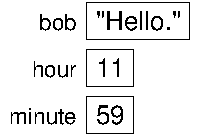
\includegraphics{assign.pdf}  %TODO replace Bob with message; draw arrow?
\end{center}

As a general rule, a variable has to have the same type as the value you assign it.
You cannot store a \java{String} in \java{minute} or an integer in \java{message}.

On the other hand, that rule can be confusing.
There are many ways that you can convert values from one type to another, and Java sometimes converts things automatically.
For now you should remember the general rule, and we'll talk about exceptions later.

Another source of confusion is that some strings {\em look} like integers, but they are not.
For example, \java{message} can contain the string \java{"123"}, which is made up of the characters \java{'1'}, \java{'2'}, and \java{'3'}.
But that is not the same thing as the number \java{123}.

\begin{code}
    bob = "123";  // legal
    bob = 123;    // not legal
\end{code}


%TODO
%\section{Constants}


\section{Printing variables}
\label{printing}

You can print the value of a variable using {\tt println} or {\tt print}:

\begin{code}
class Hello {
  public static void main(String[] args) {
    String firstLine;
    firstLine = "Hello, again!";
    System.out.println(firstLine);
  }
}
\end{code}

This program creates a variable named {\tt firstLine}, assigns it the value {\tt "Hello, again!"} and then prints that value.
When we talk about ``printing a variable,'' we mean printing the {\em value} of the variable.
To print the {\em name} of a variable, you have to put it in quotes.
For example: {\tt System.out.println("firstLine");}

For example, you can write:

\begin{code}
    String firstLine;
    firstLine = "Hello, again!";
    System.out.print("The value of firstLine is ");
    System.out.println(firstLine);
\end{code}

The output of this program is:

\begin{stdout}
The value of firstLine is Hello, again!
\end{stdout}

I am happy to report that the syntax for printing a variable is the same regardless of the variable's type.

\begin{code}
    int hour, minute;
    hour = 11;
    minute = 59;
    System.out.print("The current time is ");
    System.out.print(hour);
    System.out.print(":");
    System.out.print(minute);
    System.out.println(".");
\end{code}

%TODO
The output of this program is {\tt The current time is 11:59.}

WARNING: To put multiple values on the same line, is common to use several {\tt print} statements followed by a {\tt println}.
But you have to remember the {\tt println} at the end.
In many environments, the output from {\tt print} is stored without being displayed until {\tt println} is invoked, at which point the entire line is displayed at once.
If you omit {\tt println}, the program may terminate without displaying the stored output!


\section{Keywords}
\index{keyword}

A few sections ago, I said that you can make up any name you want for your variables, but that's not quite true.
There are certain words that are reserved in Java because they are used by the compiler to parse the structure of your program, and if you use them as variable names, it will get confused.
These words, called {\bf keywords}, include {\tt public}, {\tt class}, {\tt void}, {\tt int}, and many more.

The complete list is available at \url{http://download.oracle.com/javase/tutorial/java/nutsandbolts/_keywords.html}.
This site, provided by Oracle, includes Java documentation I refer to throughout the book.

Rather than memorize the list, I suggest you take advantage of a feature provided in many Java development environments: code highlighting.
As you type, parts of your program should appear in different colors.
For example, keywords might be blue, strings red, and other code black.
If you type a variable name and it turns blue, watch out!
You might get some strange behavior from the compiler.


\section{Arithmetic operators}
\index{operator}

{\bf Operators} are symbols used to represent computations like addition and multiplication.
Most operators in Java do what you expect them to do because they are common mathematical symbols.
For example, the operator for addition is {\tt +}.
Subtraction is {\tt -}, multiplication is {\tt *}, and division is {\tt /}.

\begin{code}
1+1        hour-1       hour*60 + minute     minute/60
\end{code}

Expressions can contain both variable names and numbers.
Variables are replaced with their values before the computation is performed.

\index{expression}

Addition, subtraction and multiplication all do what you expect, but you might be surprised by division.
For example, this program:

\begin{code}
    int hour, minute;
    hour = 11;
    minute = 59;
    System.out.print("Number of minutes since midnight: ");
    System.out.println(hour*60 + minute);
    System.out.print("Fraction of the hour that has passed: ");
    System.out.println(minute/60);
\end{code}

generates this output:

\begin{stdout}
Number of minutes since midnight: 719
Fraction of the hour that has passed: 0
\end{stdout}

The first line is expected, but the second line is odd.
The value of {\tt minute} is 59, and 59 divided by 60 is 0.98333, not 0.
The problem is that Java is performing {\bf integer division}.

\index{type!int}
\index{integer division}
\index{arithmetic!integer}
\index{division!integer}
\index{operand}

When both {\bf operands} are integers (operands are the things operators operate on), the result is also an integer, and by convention integer division always rounds {\em down}, even in cases like this where the next integer is so close.

An alternative is to calculate a percentage rather than a fraction:

\begin{code}
    System.out.print("Percentage of the hour that has passed: ");
    System.out.println(minute*100/60);
\end{code}

The result is:

\begin{stdout}
Percentage of the hour that has passed: 98
\end{stdout}

Again the result is rounded down, but at least now the answer is approximately correct.
To get a more accurate answer, we can use a different type of variable, called floating-point, that can store fractional values.
We'll get to that in the next chapter.


\section{Order of operations}
\index{precedence}
\index{order of operations}

When more than one operator appears in an expression, the order of evaluation depends on the rules of {\bf precedence}.
A complete explanation of precedence can get complicated, but just to get you started:

\begin{itemize}

\item Multiplication and division happen before addition and subtraction.
So {\tt 2*3-1} yields 5, not 4, and {\tt 2/3-1} yields -1, not 1 (remember that in integer division {\tt 2/3} is 0).

\item If the operators have the same precedence they are evaluated from left to right.
So in the expression {\tt minute*100/60}, the multiplication happens first, yielding {\tt 5900/60}, which in turn yields {\tt 98}.
If the operations had gone from right to left, the result would be {\tt 59*1} which is {\tt 59}, which is wrong.

\item Any time you want to override the rules of precedence (or you are not sure what they are) you can use parentheses.
Expressions in parentheses are evaluated first, so {\tt 2 *(3-1)} is 4.
You can also use parentheses to make an expression easier to read, as in {\tt(minute * 100) / 60}, even though it doesn't change the result.

\end{itemize}


\section{Operators for {\tt Strings}}

\index{string operator}
\index{operator!string}

In general you cannot perform mathematical operations on {\tt String}s, even if the strings look like numbers.
The following are illegal (if we know that bob has type {\tt String}):

\begin{stdout}
bob - 1         "Hello"/123      bob * "Hello"
\end{stdout}

By the way, can you tell by looking at those expressions whether {\tt bob} is an integer or a string?
Nope.
The only way to tell the type of a variable is to look at the place where it is declared.

\index{concatenate}

Interestingly, the {\tt +} operator {\em does} work with {\tt String}s, but it might not do what you expect.
For {\tt String}s, the {\tt +} operator represents {\bf concatenation}, which means joining up the two operands by linking them end-to-end.
So {\tt "Hello, " + "world."} yields the string {\tt "Hello, world."} and {\tt bob + "ism"} adds the suffix {\em ism} to the end of whatever {\tt bob} is, which is handy for naming new forms of bigotry.


\section{Composition}

\index{composition}
\index{expression}

So far we have looked at the elements of a programming language---variables, expressions, and statements---in isolation, without talking about how to combine them.

One of the most useful features of programming languages is their ability to take small building blocks and {\bf compose} them.
For example, we know how to multiply numbers and we know how to print; it turns out we can combine them in a single statement:

\begin{code}
    System.out.println(17 * 3);
\end{code}

Any expression involving numbers, strings and variables, can be used inside a print statement.
We've already seen one example:

\begin{code}
    System.out.println(hour*60 + minute);
\end{code}

But you can also put arbitrary expressions on the right-hand side of an assignment statement:

\begin{code}
    int percentage;
    percentage = (minute * 100) / 60;
\end{code}

This ability may not seem impressive now, but we will see examples where composition expresses complex computations neatly and concisely.

WARNING: The left side of an assignment has to be a {\em variable} name, not an expression.
That's because the left side indicates the storage location where the result will go.
Expressions do not represent storage locations, only values.
So the following is illegal: {\tt minute+1 = hour;}.


\section{Readability and style}

As a rule of thumb, each line should be one statement / action.

TODO

Static analysis with Checkstyle
